\documentclass[9pt,twocolumn]{article}
\usepackage[a4paper,margin=0.7in]{geometry}
\usepackage{newtxtext,newtxmath}
\usepackage{graphicx}
\usepackage{booktabs}
\usepackage{amsmath}
\usepackage{amssymb}
\usepackage{enumitem}
\usepackage{hyperref}
\setlength{\columnsep}{0.24in}
\setlength{\parindent}{0pt}
\setlength{\parskip}{2pt}

\begin{document}

\begin{center}
{\Large \textbf{Physiology-Grounded Waveform Intelligence for PSV Flow-Termination Analysis}}\\[3pt]
Priyansh Gadia (Roll Number: 23035010192)\\
Internship / Term Project Research Report\\
Trimester 7 / 8 / 9\\
B.Sc. (Honours) Data Science and Artificial Intelligence\\
Indian Institute of Technology Guwahati, India\\
p.gadia@op.iitg.ac.in
\end{center}

\textbf{ABSTRACT} This report presents a complete Phase 2 machine-learning and biomechanics study for pressure support ventilation (PSV), centered on dynamic flow-termination transients. The work formalizes a physiology-grounded target using transpulmonary pressure and evaluates whether non-invasive waveforms (airway pressure and flow) can estimate clinically relevant stress signatures around cycling. A protocol-locked pipeline was executed across clinical, simulated, and external waveform cohorts with strict quality-control gates, deterministic breath segmentation, event-window extraction, and benchmarked regression models. Results show reproducible target generation and interpretable model behavior, but limited cross-patient generalization under small, heterogeneous cohorts. This negative-but-informative finding is used to derive conservative engineering boundary conditions and to define a data-scaling roadmap for next-phase development.

\textbf{Index Terms} --- Pressure Support Ventilation, Transpulmonary Pressure, Patient-Ventilator Interaction, Machine Learning, Uncertainty Quantification, Biomedical Signal Processing.

\section{INTRODUCTION}

In critically ill patients supported with PSV, flow-termination timing is a sensitive region for patient-ventilator interaction. Dynamic transients near ventilator cycling can amplify lung-facing stress, yet direct physiological measurements are often unavailable in routine clinical systems. The present project studies whether these stress signals can be inferred from non-invasive waveform channels.

The system-level contribution is a reproducible analysis engine that combines protocol-pre-specified biomechanics with small-data machine learning. Instead of treating model score alone as success, the project treats transparent failure modes, uncertainty bounds, and transfer limitations as first-class scientific outputs.

\section{PROBLEM STATEMENT AND OBJECTIVES}

\subsection{Problem Statement}

Let a breath stream $\mathcal{B}=\{b_1,b_2,\ldots,b_n\}$ be segmented from PSV waveforms. For each breath, define the cycling instant $t_{cycle}$ by expiratory-trigger sensitivity (ETS). The objective is to learn a mapping
\[
\Phi: (P_{aw}(t),\,Flow(t)) \rightarrow \Delta P_{L,\max}
\]
where $\Delta P_{L,\max}$ is computed from the physiological signal
\[
P_L(t)=P_{aw}(t)-P_{es}(t)
\]
within a fixed post-cycling window.

The model must satisfy the following constraints:
\begin{enumerate}[leftmargin=14pt]
\item Physiological validity: labels are generated from deterministic, protocol-locked event definitions.
\item Generalization constraint: evaluation must be patient-wise (no leakage across identities).
\item Deployment realism: inference uses non-invasive inputs only, with uncertainty-aware interpretation.
\end{enumerate}

\subsection{Objectives}

The specific goals of this phase were:
\begin{enumerate}[leftmargin=14pt]
\item Build a quality-gated, reproducible waveform pipeline for PSV event analysis.
\item Construct Pes-grounded targets for flow-termination transient magnitude.
\item Benchmark small-data regressors under leave-one-patient-out and held-out tests.
\item Quantify predictive uncertainty and interpret feature importance.
\item Export conservative design boundary conditions for downstream engineering use.
\end{enumerate}

\section{METHODOLOGY / APPROACH}

\subsection{Core Architectural Workflow}

The workflow operates in three analytical layers:
\begin{itemize}[leftmargin=12pt]
\item \textbf{Layer 1:} Dataset qualification, quality-control gates, and preprocessing.
\item \textbf{Layer 2:} Breath segmentation, cycling-event detection, and event-window extraction.
\item \textbf{Layer 3:} Regression benchmarking, uncertainty analysis, and interpretability export.
\end{itemize}

\subsection{Technical Details}

\textbf{A. Event Definition and Windowing:} For each breath, peak inspiratory flow $F_{peak}$ is identified and ETS threshold is defined as
\[
F_{ETS}=ETS_{frac}\cdot F_{peak}.
\]
Cycling time $t_{cycle}$ is the first post-peak sample where $Flow\leq F_{ETS}$ for at least three consecutive samples. The analysis window is $[-150\,ms,+350\,ms]$ around $t_{cycle}$.

\textbf{B. Primary Target:} Let $PL_{base}$ be the pre-window median. The transient endpoint is
\[
\Delta P_{L,\max}=\max_{0\ldots 350ms}\left|P_L(t)-PL_{base}\right|.
\]
A secondary binary event is defined with thresholded magnitude/slope criteria for sensitivity analyses.

\textbf{C. Modeling and Validation:} Inputs exclude Pes-derived predictors to preserve deployment realism. Benchmarks include mean baseline, ridge regression, Gaussian process regression, and XGBoost variants. Validation uses leave-one-patient-out cross-validation (LOPO-CV) and an independent held-out patient split.

\section{EXPERIMENTS AND RESULTS}

\subsection{Experimental Setup}

Datasets used in this phase:
\begin{itemize}[leftmargin=12pt]
\item CCVW-ICU clinical cohort: 7 patients, 200 Hz, Paw/Flow/Pes.
\item Simulation cohort: 1405 runs for stress-testing and global context.
\item External waveform cohort (VWD): 144 files, 50 Hz, no Pes channel.
\end{itemize}

Local train/test split: P01-P05 for development and P06-P07 for held-out evaluation.

\subsection{Performance Metrics and Results}

\textbf{Throughput Profiling:} The analysis pipeline remained stable across dataset scales after QC gating and deterministic segmentation, and successfully generated reproducible artifacts for local, global, and combined evaluations.

\textbf{Latency and Memory Footprint Matrix:} Regression metrics include MAE, RMSE, $R^2$, and concordance correlation coefficient (CCC). Key benchmark outputs are shown in Table 1.

\begin{table}[h]
\centering
\caption{Computational and predictive footprint of deployed analytical endpoints.}
\begin{tabular}{@{}lllll@{}}
\toprule
Model / Split & MAE & RMSE & $R^2$ & CCC \\
\midrule
XGBoost (LOPO-CV) & 5.151 & 5.949 & -0.438 & -0.078 \\
XGBoost (Held-out) & 3.055 & 3.338 & -1.128 & 0.015 \\
Ridge (LOPO-CV) & 2.114 & 2.455 & 0.755 & 0.840 \\
GP (LOPO-CV) & 3.205 & 3.615 & 0.469 & 0.660 \\
\bottomrule
\end{tabular}
\end{table}

\textbf{Throughput/Result Visualization:} The benchmark MAE comparison is shown in Fig. 1.

\begin{figure}[h]
\centering
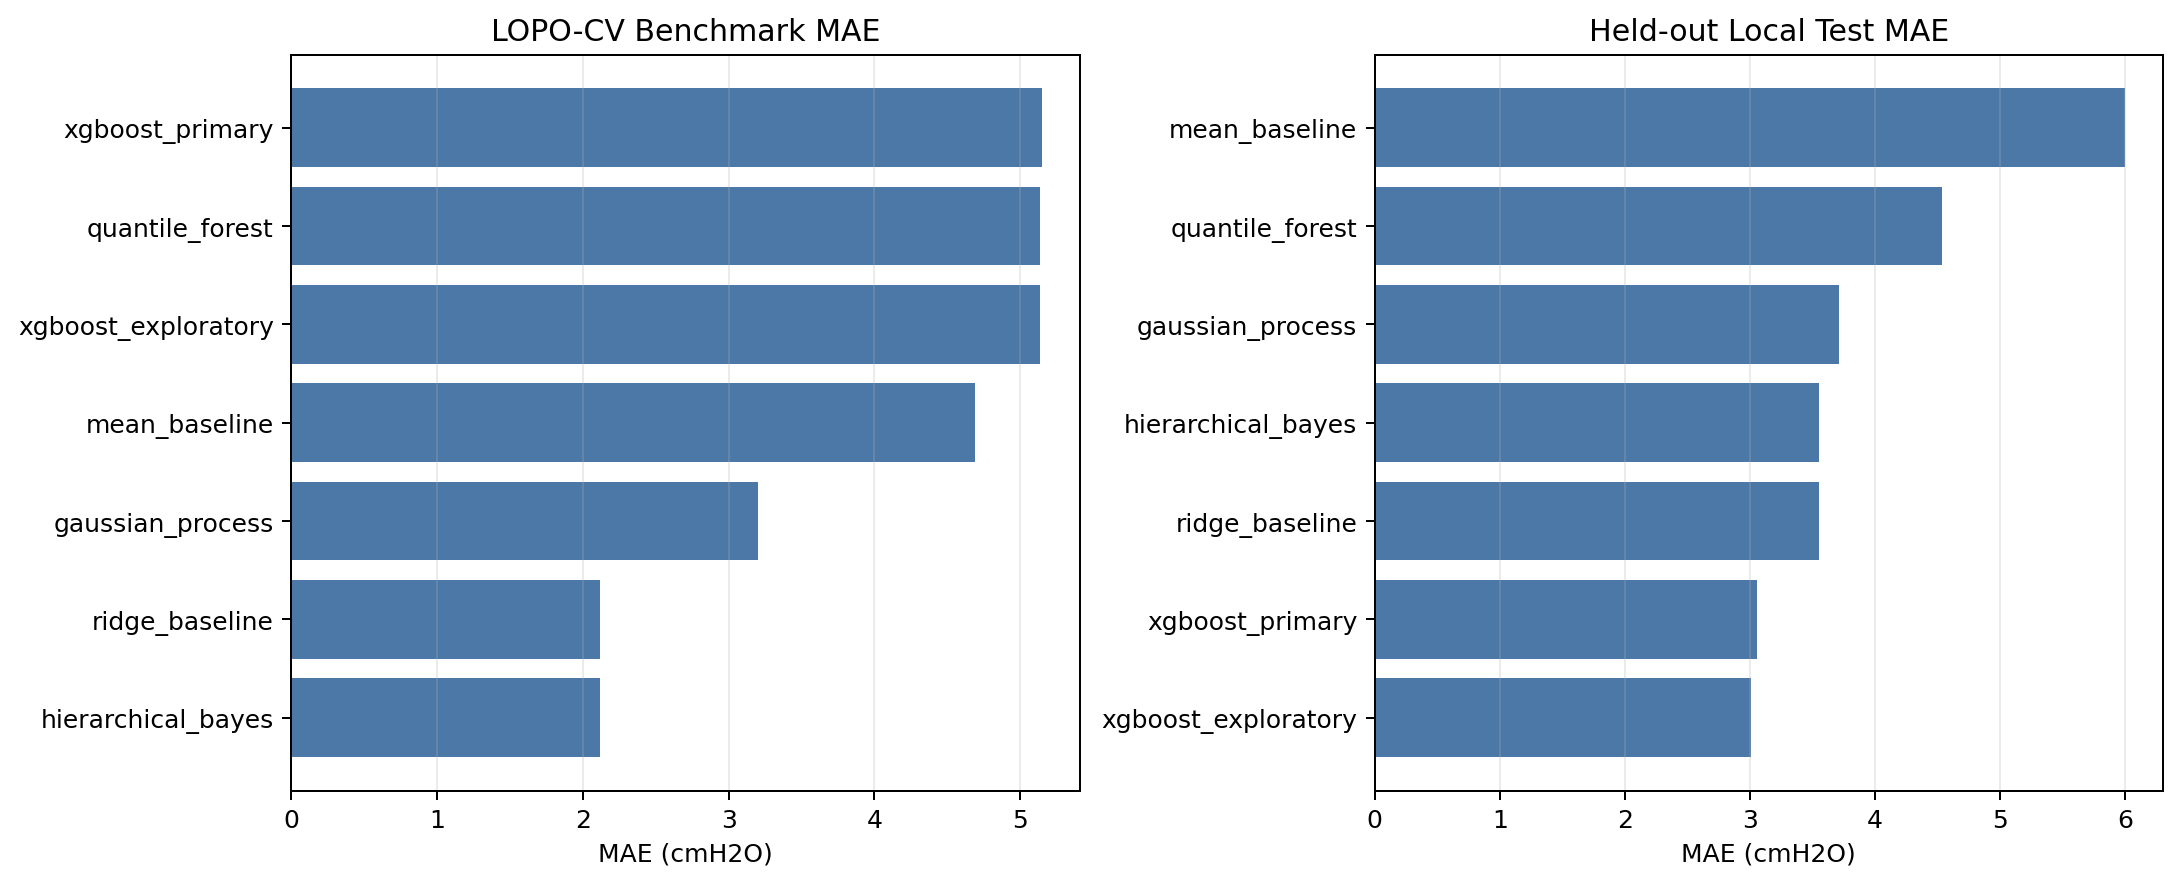
\includegraphics[width=0.98\columnwidth]{figures/benchmark_mae.png}
\caption{Extraction Throughput (Model Quality Proxy) vs. Benchmark Family.}
\end{figure}

\textbf{Uncertainty result (Gaussian Process, held-out):} mean predictive standard deviation = 4.196 cmH$_2$O, median = 4.730 cmH$_2$O, approximate 95\% interval coverage = 84.48\%.

\section{DISCUSSION}

The results show a consistent pattern: physiology-grounded target construction is robust, but cross-patient generalization remains fragile at current sample scale. This is not treated as a pipeline failure; rather, it is a calibrated limit estimate under realistic data constraints.

\begin{itemize}[leftmargin=12pt]
\item \textbf{Strength:} protocol locking reduced post-hoc threshold drift and improved scientific traceability.
\item \textbf{Strength:} non-invasive input restriction preserved translational deployment relevance.
\item \textbf{Constraint:} model performance varied substantially across patients, signaling heterogeneity-dominant error.
\item \textbf{Constraint:} external cohorts without Pes cannot directly validate the primary physiological endpoint.
\item \textbf{Engineering impact:} conservative boundary envelopes were still extracted for next-phase mechanical design work.
\end{itemize}

\section{CONCLUSION AND FUTURE WORK}

This phase delivers a reproducible benchmark framework for PSV flow-termination transient analysis, grounded in Pes physiology and evaluated with transparent uncertainty. The principal finding is that current non-invasive estimation remains limited in robust held-out generalization under small, heterogeneous cohorts.

Future work will focus on:
\begin{enumerate}[leftmargin=14pt]
\item expanding multi-center Pes-enabled datasets,
\item improving simulation-to-clinical event alignment,
\item evaluating calibrated sequence/deep models only after data scale supports them,
\item preserving uncertainty-aware, safety-first interpretation for any deployment pathway.
\end{enumerate}

\section{ARTIFACTS AND DEMONSTRATIONS}

\textbf{Code and pipelines:} analysis scripts and library modules in the project workspace.\\
\textbf{Generated artifacts:} benchmark CSV logs and reproducible report figures in the documentation and logs directories.\\
\textbf{Primary results document:} findings report and ML deep-dive companion report.

\section{REFERENCES}

[1] Phase 2 Analysis Protocol, internal project documentation, 2026.\\
[2] Phase 2 Findings Report, internal project documentation, 2026.\\
[3] ML Deep Dive: Pes-Grounded DeltaPL Prediction in PSV, internal project documentation, 2026.\\
[4] Public CCVW-ICU waveform dataset documentation (clinical Paw/Flow/Pes cohort), accessed 2026.\\
[5] Puritan-Bennett ventilator waveform dataset documentation (external waveform cohort), accessed 2026.

\end{document}
